\documentclass[USenglish]{article}

%\usepackage[utf8]{inputenc}%(only for the pdftex engine)
\RequirePackage[no-math]{fontspec}[2017/03/31]%(only for the luatex or the xetex engine)
\usepackage[small]{dgruyter}

\usepackage{natbib}
\bibliographystyle{apalike}

\usepackage{microtype}

\begin{document}

  \articletype{Research Article}

  \author*[1]{C.J.(Chaojie) Duan}
  %\author[2]{...}
  %\author[1]{...} 
  \runningauthor{Duan}
  \affil[1]{Dulun Consulting Group, research@dulun.com}
  %\affil[2]{...}
  \title{How Much Does Home-Field Advantage Matter in Professional Soccer?}
  \runningtitle{Bayesian Hierarchical Analysis}
  \subtitle{A Multilevel Bayesian Investigation}
  \abstract{Using 2001 to 2017 seasonal data,, we fit a Bayesian multilevel nested model to the parameters in a Home-Field Advantage (HFA) model, allowing information obtained from the team level to inform the inferences at the upper league and sport levels.}
  \keywords{European Professional Soccer Leagues, Home Field Advantage, Poisson generative process, Stan}
  %\classification[PACS]{...}
  %\communicated{...}
  %\dedication{...}
  \received{5/21/2018}
  %\accepted{...}
  \journalname{Journal of Quantitative Analysis in Sports}
  %\journalyear{...}
  %\journalvolume{..}
  %\journalissue{..}
  \startpage{1}
  %\aop
  %\DOI{...}
\maketitle

\section{Introduction} 

%The National Football League is tapping Amazon Web Services to help power its “Next Gen Stats” platform.
%Aiming to uncover deeper insights into the games of professional football, the National Football League (NFL) recently announced that it will be powering its Next Gen Stats with Amazon's Cloud Computing Platform - AWS to kick off the 2018 season. %with more impactful and meaningful content.  
%Amazon’s cloud computing arm also powers Statcast, the next generation statistics platform for Major League Baseball (MLB). These high-profile tech-sport partnerships are arguably the latest and most visible account of invasion of analytics into the realms of spectator sports.

In professional team sports, the term home field advantage (HFA) – also called home advantage, home ground or home court advantage, defender's advantage, home-ice advantage – describes the benefit that the home team is believed to gain over the visiting opponent. Its scientific definition is ``the consistent finding that home teams in sport competition win over 50\% of the games played under s balanced home and away schedule'' \citep[p. 13]{Courneya1992}.
Due to the existence of HFA, many vital games, such as playoff or elimination matches, in major professional sports have special rules for determining which match is played at which place. In particular,  the Union of European Football Associations (UEFA) institutionalized the ruling that a second leg of any Champions League knock-off series is favorable to playing away with the the scores still in balance after the first leg competition \citep{atkins2013}.
\begin{figure}[ht]
\caption{\textit{Revenue of the top European soccer leagues (Big Five*) from 2006/07 to 2016/17 (in billion euros)}}

\centering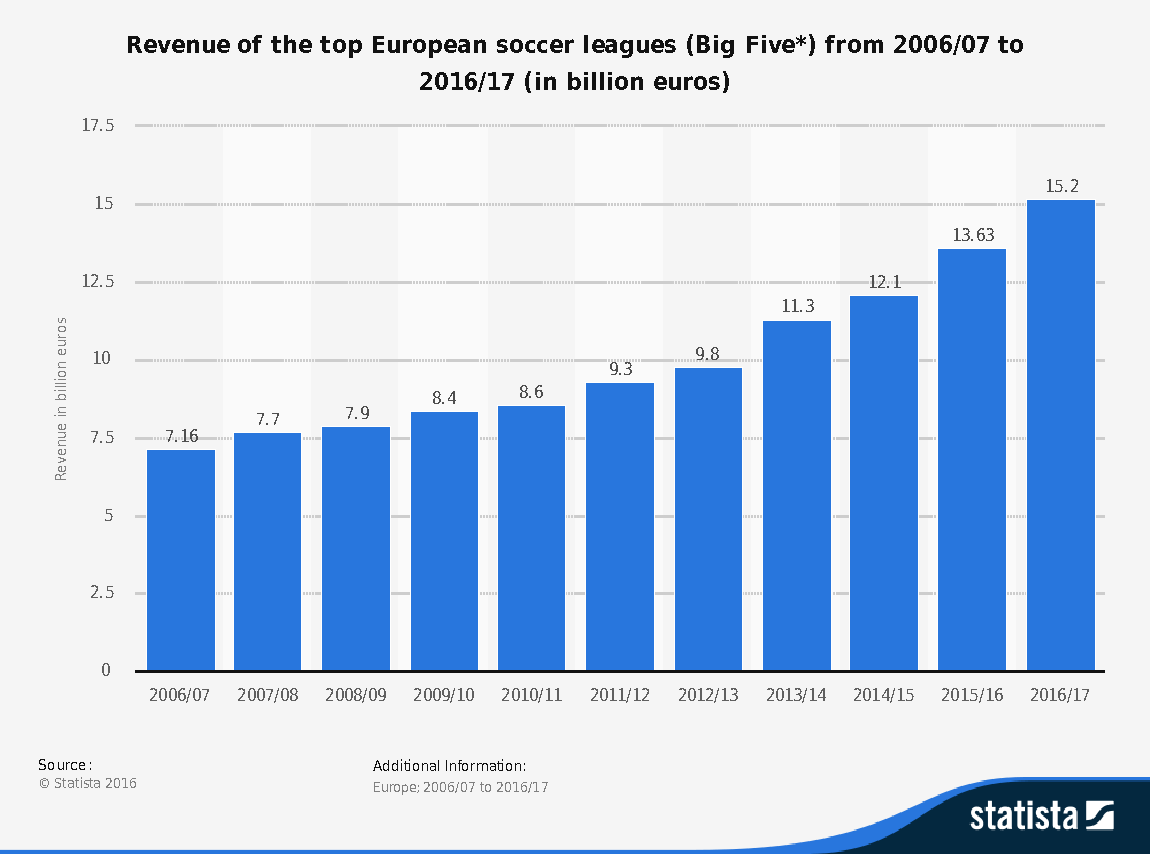
\includegraphics[width=0.8\textwidth]{HFA11.pdf}
\label{fig11}
\end{figure}


%Accompanying the wide-spreading notoriety in the general populace is the ever-increasing availability and volume of data associated with games, players, teams, and sports.   

%a new platform that uses data from player and ball tracking devices to produce new advanced statistics like distance covered, speed, and acceleration — the idea is to better show a receiver’s ability to get open, for example, or how well the offensive line protects the quarterback. The information is shown to fans online and on TV broadcasts; teams also leverage the data internally for strategic purposes.

%we’ll be able to kick off our 2018 season with even more impactful and meaningful content, uncovering deeper insights into the game of football than we’ve ever done before,” 

%Matt Swensson, vice president of emerging products and technology at the NFL, said in a statement. “We chose AWS because of its combination of advanced cloud offering, powerful machine learning capabilities, and experience operating at the scale we need.”





%The popular frequentist (Fisherian) statistical inference process starts with the formulation of an alternative research hypothesis(Ha), such as "people with higher income live happier than low income earners", which is typically set up against a null non-effect hypothesis (Ho), such as ``income level has no effect on happiness". Then researchers collect relevant data (each subject's perceived happiness and income), and conduct a statistical. 

%\citep{Gajewski2006}
%\citep{Carron2005}

 


A second motivator for this study is related to the hotly debated topic of home field advantage (HFA) in soccer competition. The contributions we made in this paper are (1) highlighting the different generative process underlying most sports performance metrics and suggesting corresponding solutions.  (2) investigating the long and firmly held belief of HFA simultaneously at sport, league, team levels. (3) using season performance data to rule out incidental game specifics.
 
\section{Review of Literature} 

%-----------------------
 
%=====================================================

\section{Data and Analyses} 

\begin{figure}
\caption{The Hierarchical Model of Home Field Advantage }
{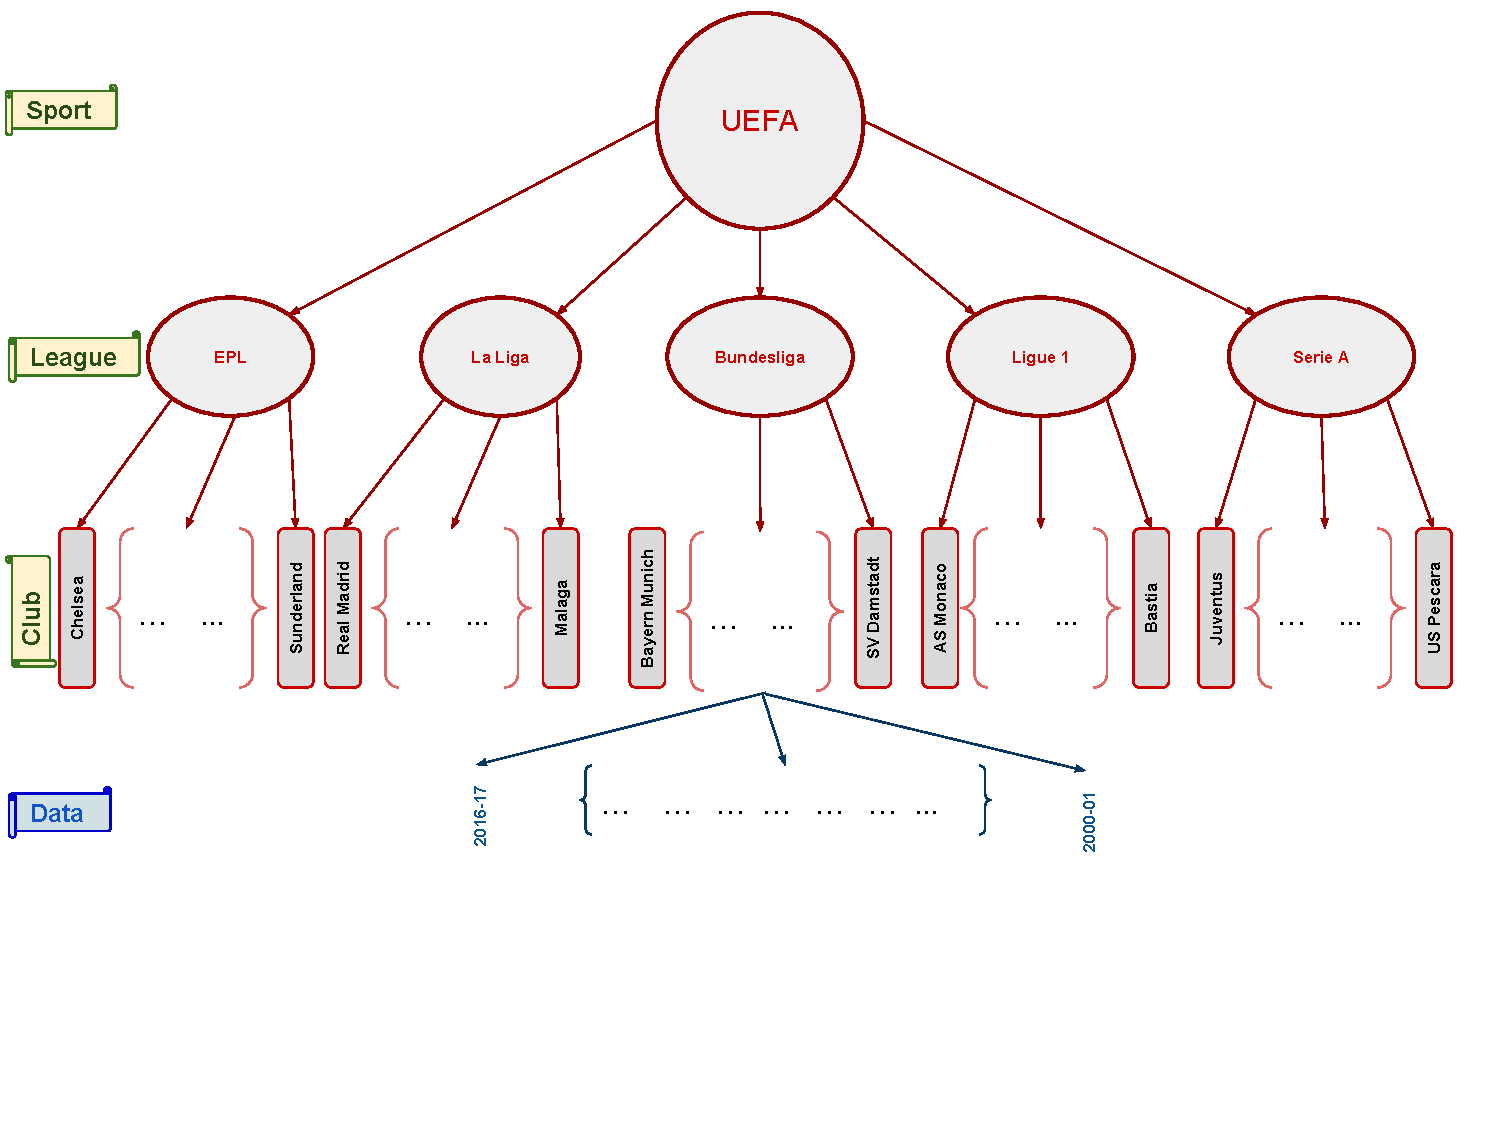
\includegraphics[width=1.0\linewidth]{HFA_Model1.pdf}}
\label{fig21}
\end{figure} 
 

\subsection{Sources} 



%-----------------------
\begin{table}[ht]
\caption{Descriptive Statistics}
\centering
\begin{tabular}{cccccccc}
\starttabularbody
\hline 
 & Mean & Median & Std. Dev. & Min. & Max. & Skewness & Kurtosis\\
\hline
 MHG & 3.634 & 4 & 1.676 & 0 & 9 & 0.246 & 0.034 \\
\hline 
 MAG & 2.884 & 3 & 1.676 & 0 & 10 & 0.627 & 0.786 \\
\hline
\end{tabular}
\label{tab1}
%{Goal Scoring Metrics: Most Home \& Away Goals at the Season Level} 
\end{table}
%=====================================================
\subsection{Results} 


\begin{figure}
\caption{Home Field Advantage Posterior Plot at Sport and League Levels}
{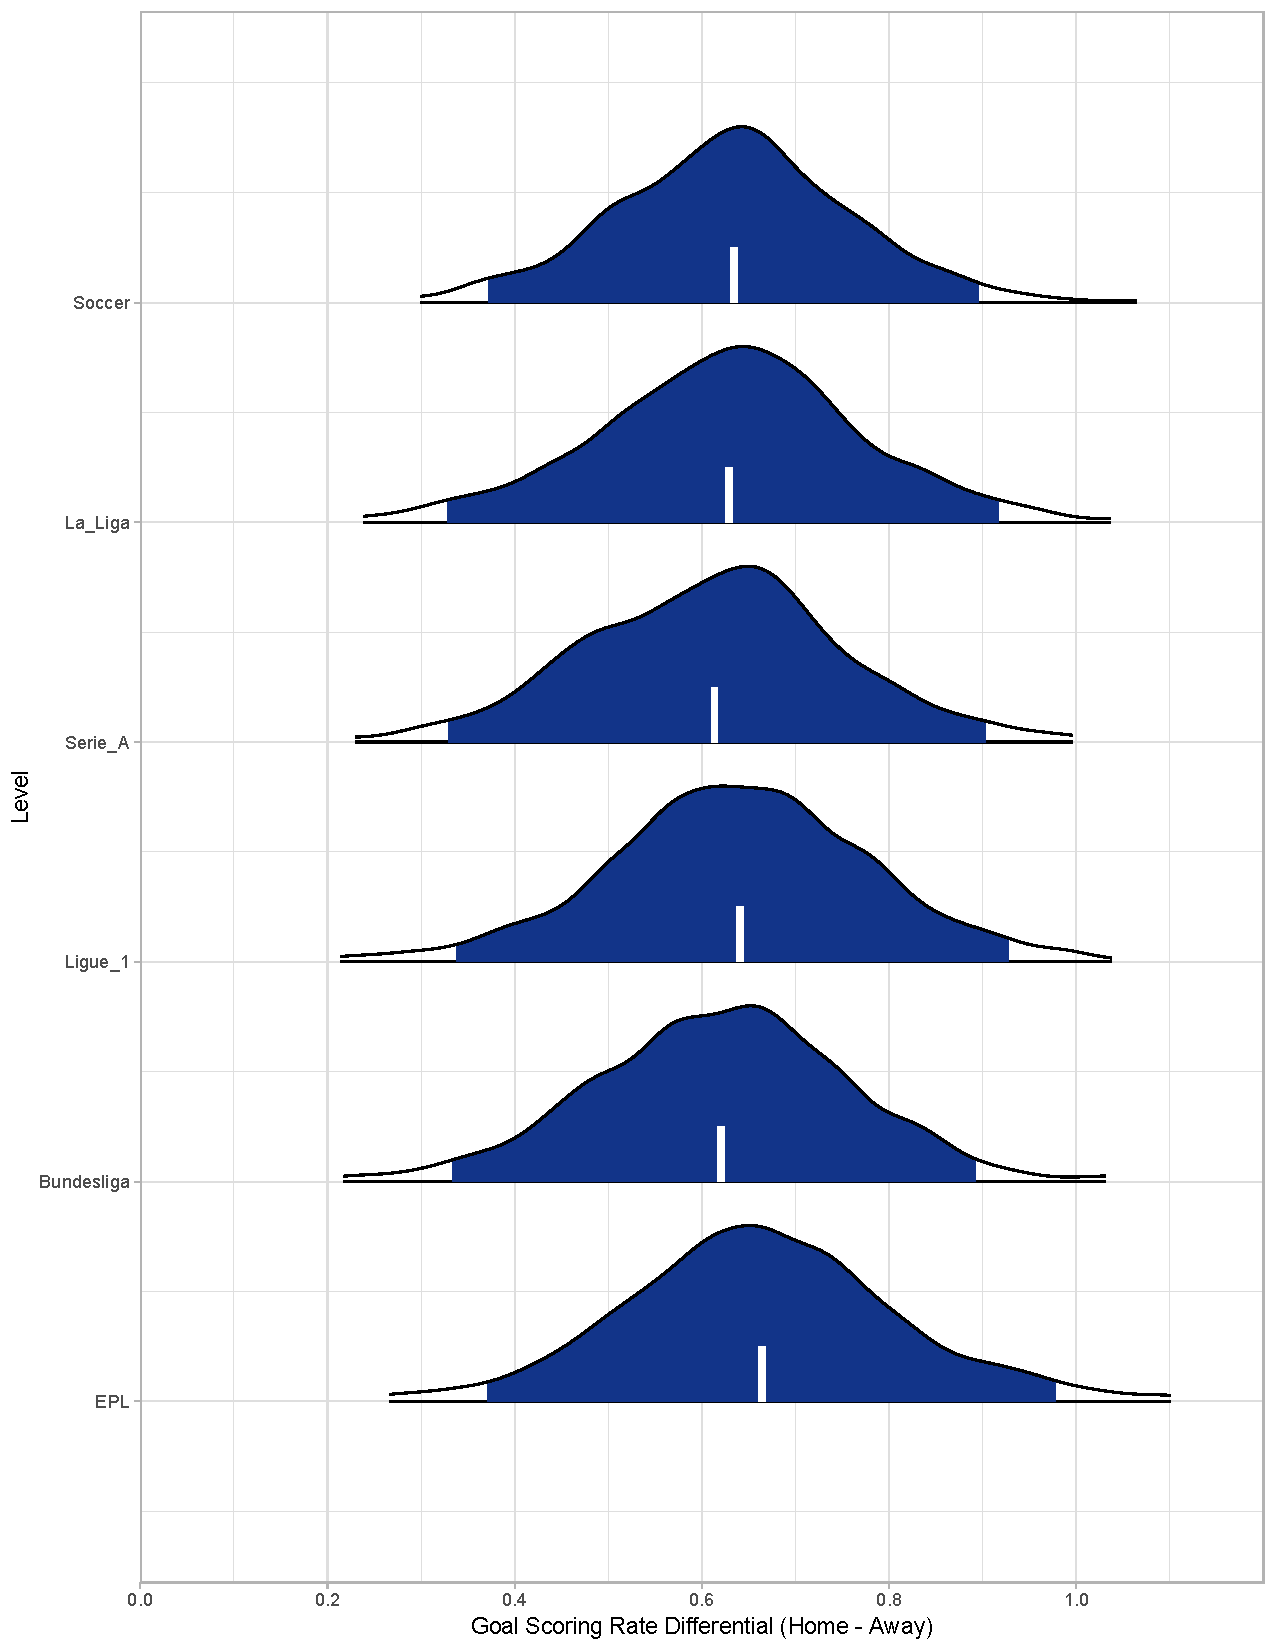
\includegraphics[width=0.80\linewidth]{HFA32.pdf}}
\label{fig2}
\end{figure}

\begin{figure}
\caption{Home Field Advantage Posterior Plot for La Liga Teams}
{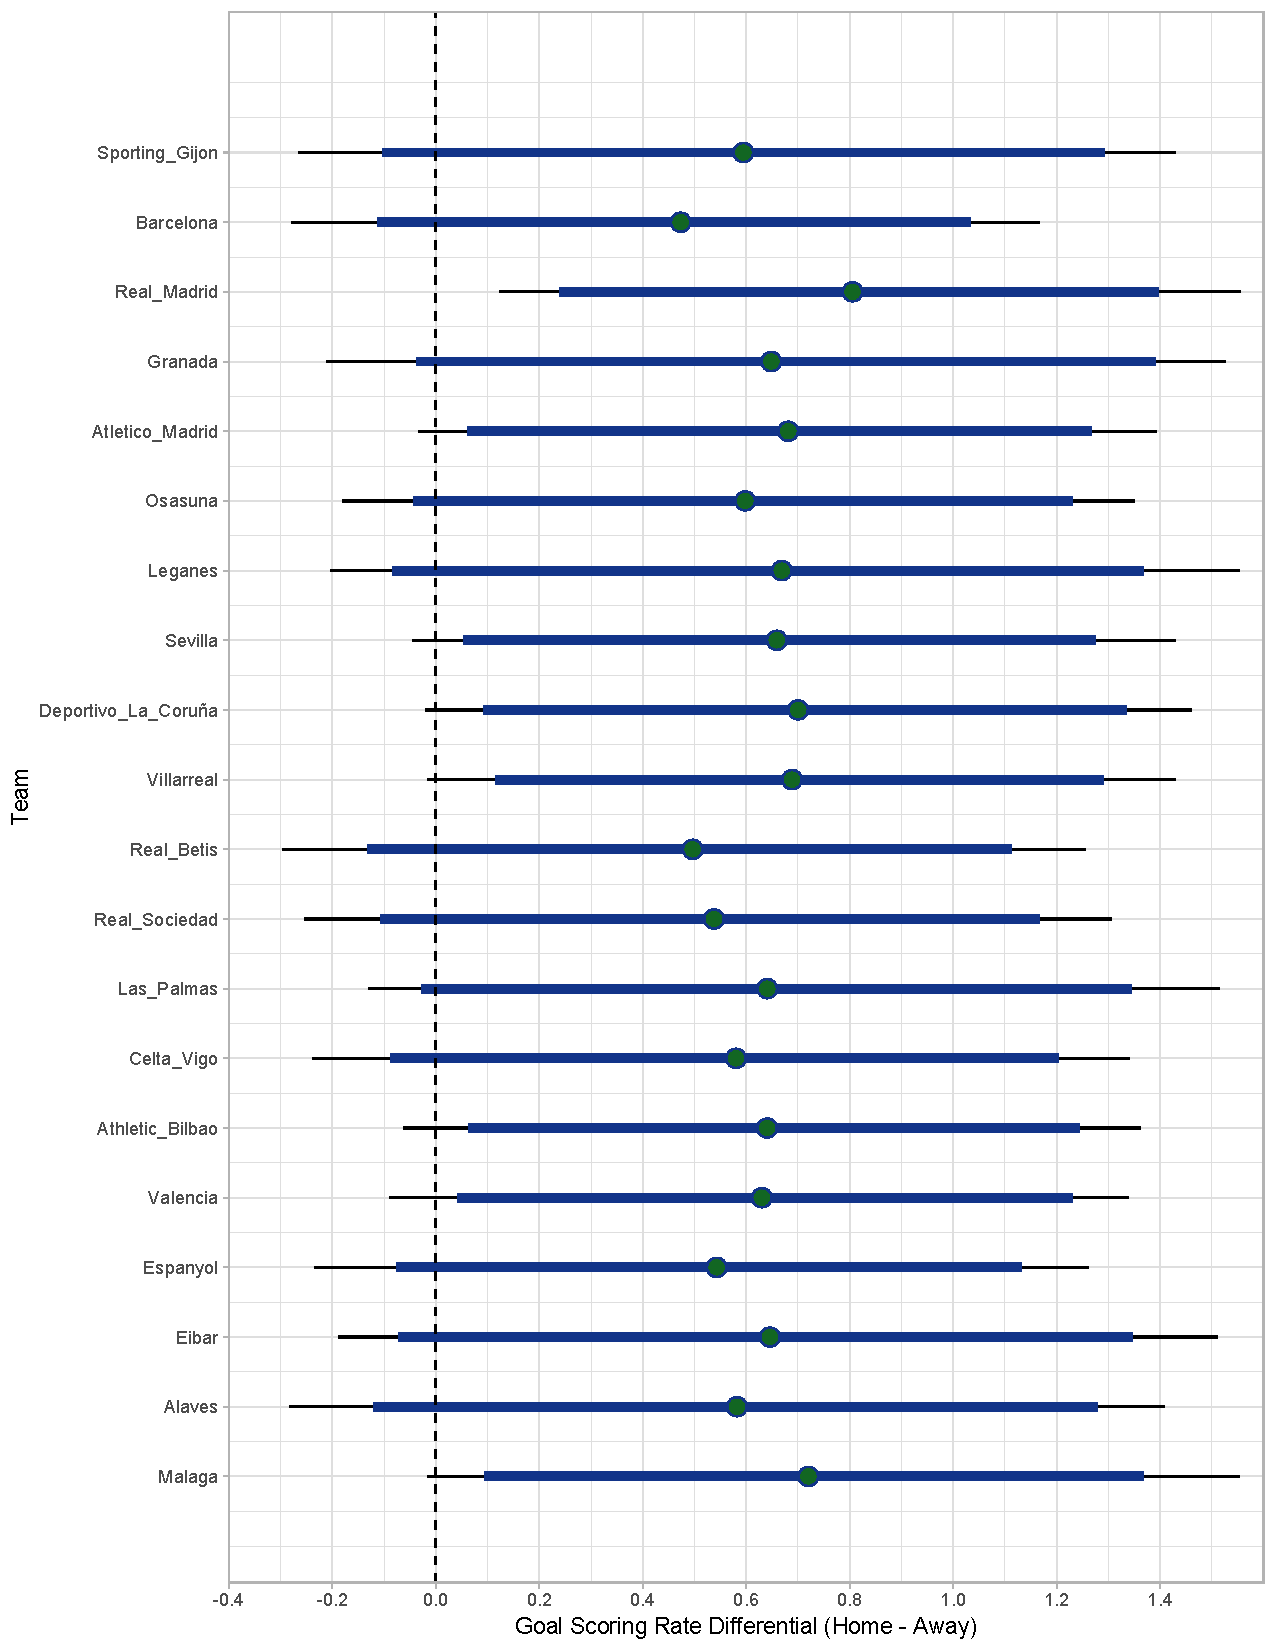
\includegraphics[width=0.90\linewidth]{HFA_La_Liga11.pdf}}
\label{fig3}
\end{figure}


\begin{figure}
\caption{Home Field Advantage Posterior Plot for Serie A Teams}
{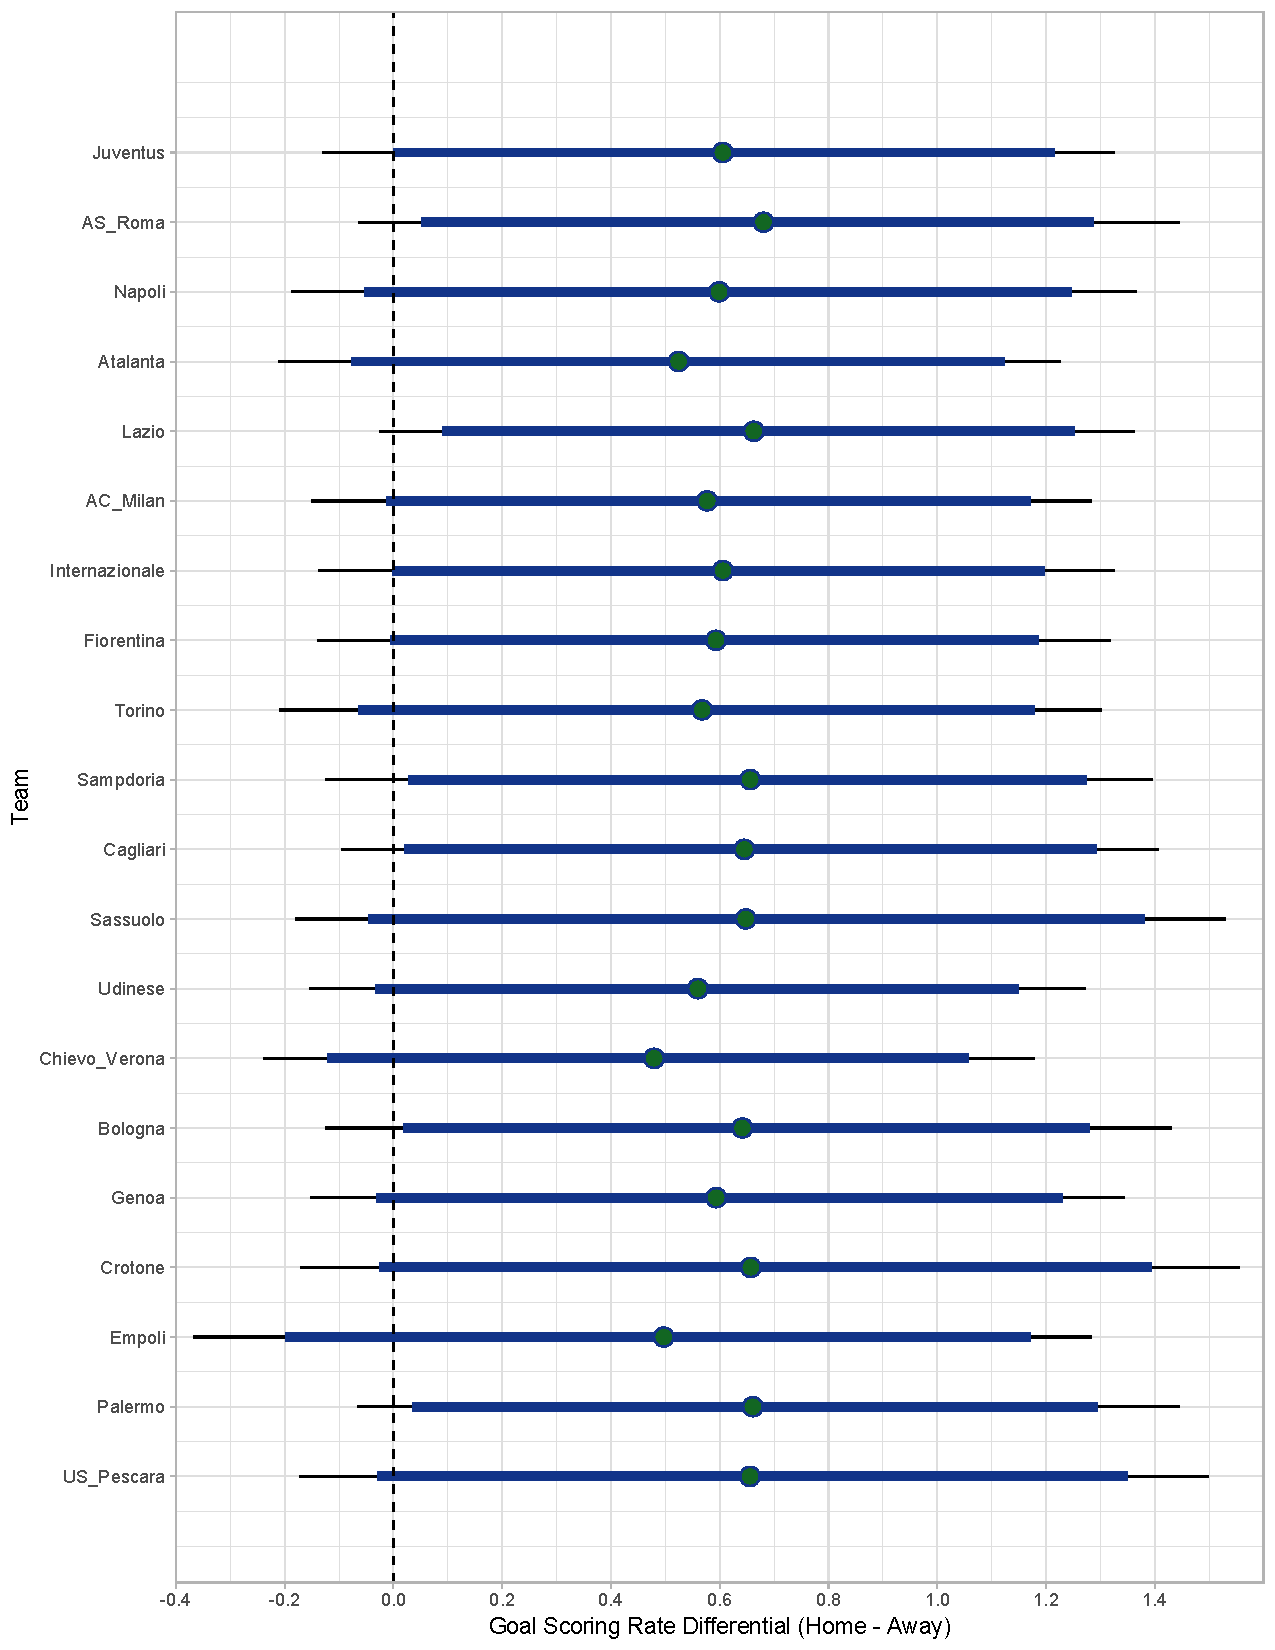
\includegraphics[width=0.90\linewidth]{HFA_Serie_A11.pdf}}
\label{fig4}
\end{figure}

\begin{figure}
\caption{Home Field Advantage Posterior Plot for Ligue 1 Teams}
{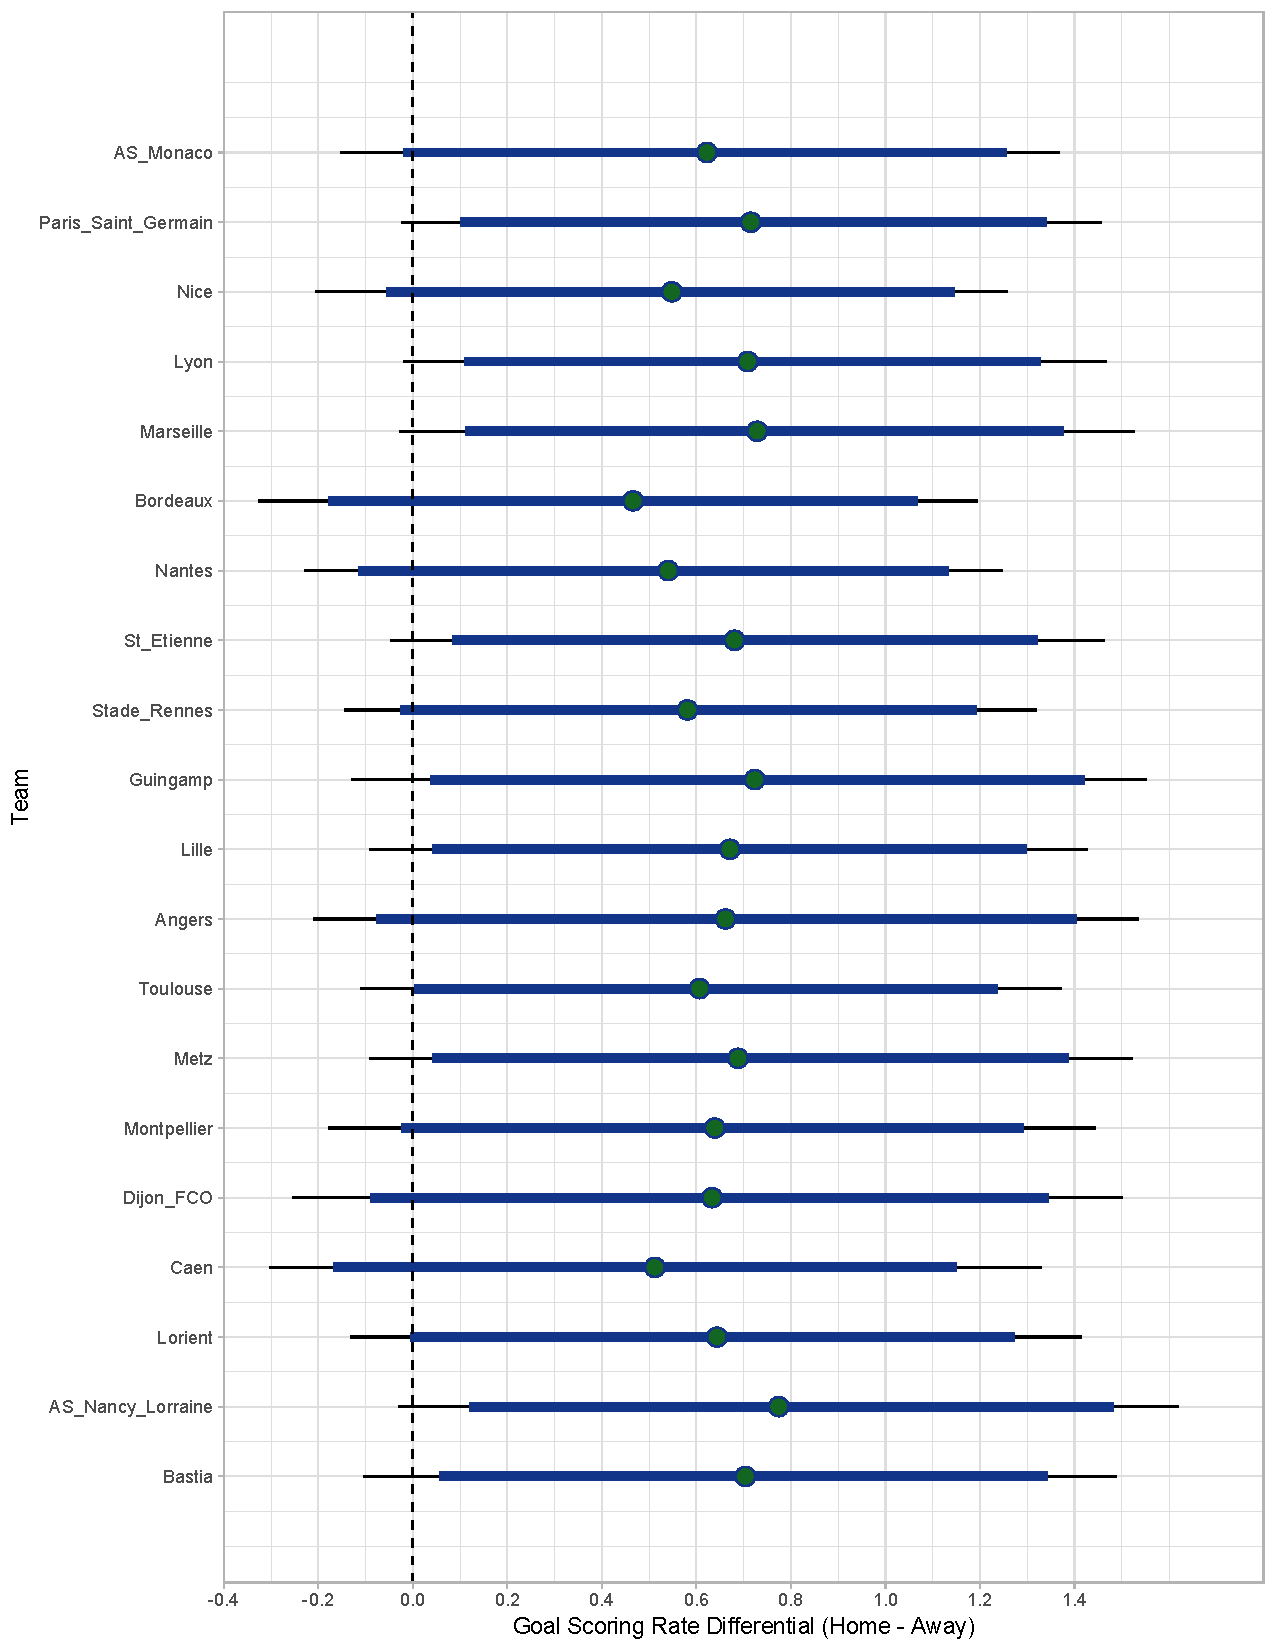
\includegraphics[width=0.90\linewidth]{HFA_Ligue111.pdf}}
\label{fig5}
\end{figure}

\begin{figure}
\caption{Home Field Advantage Posterior Plot for Bundesliga Teams}
{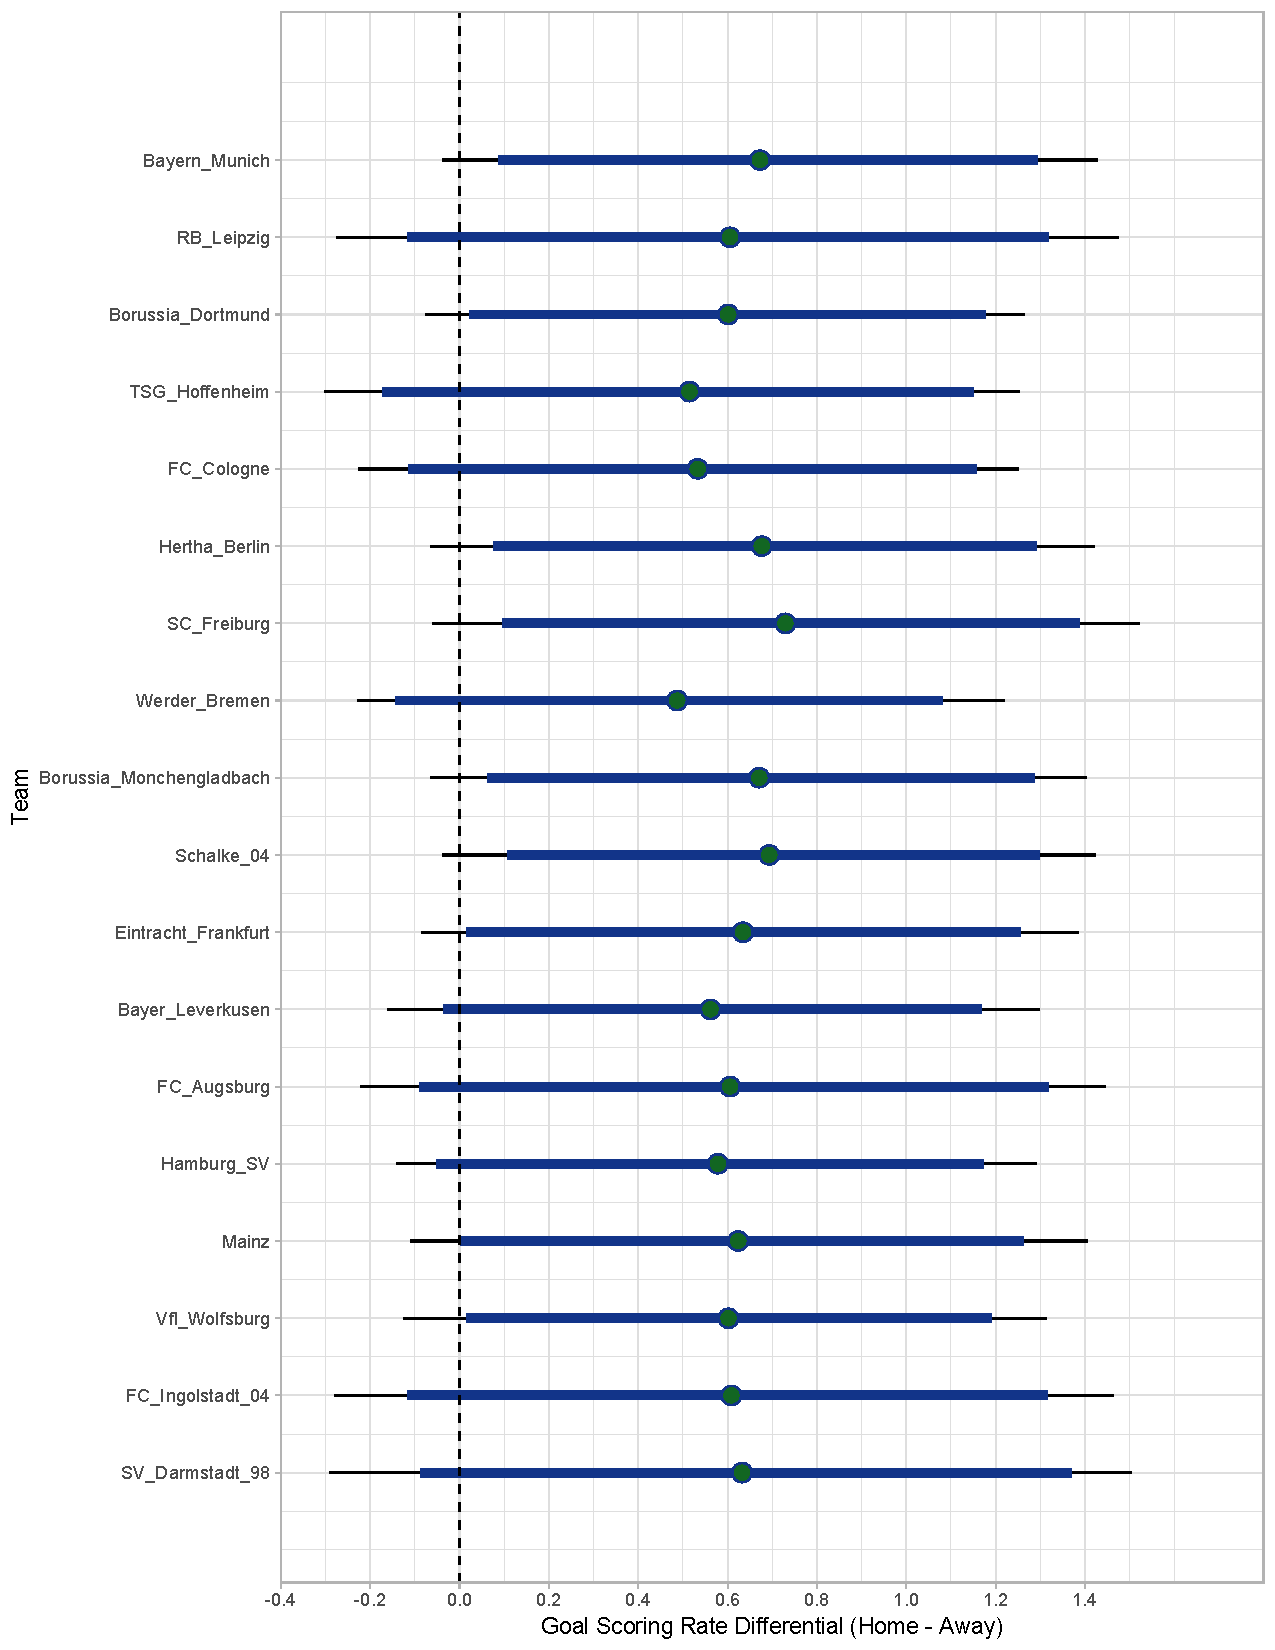
\includegraphics[width=0.90\linewidth]{HFA_Bundesliga11.pdf}}
\label{fig6}
\end{figure}

\begin{figure}
\caption{Home Field Advantage Posterior Plot for English Premier League Teams}
{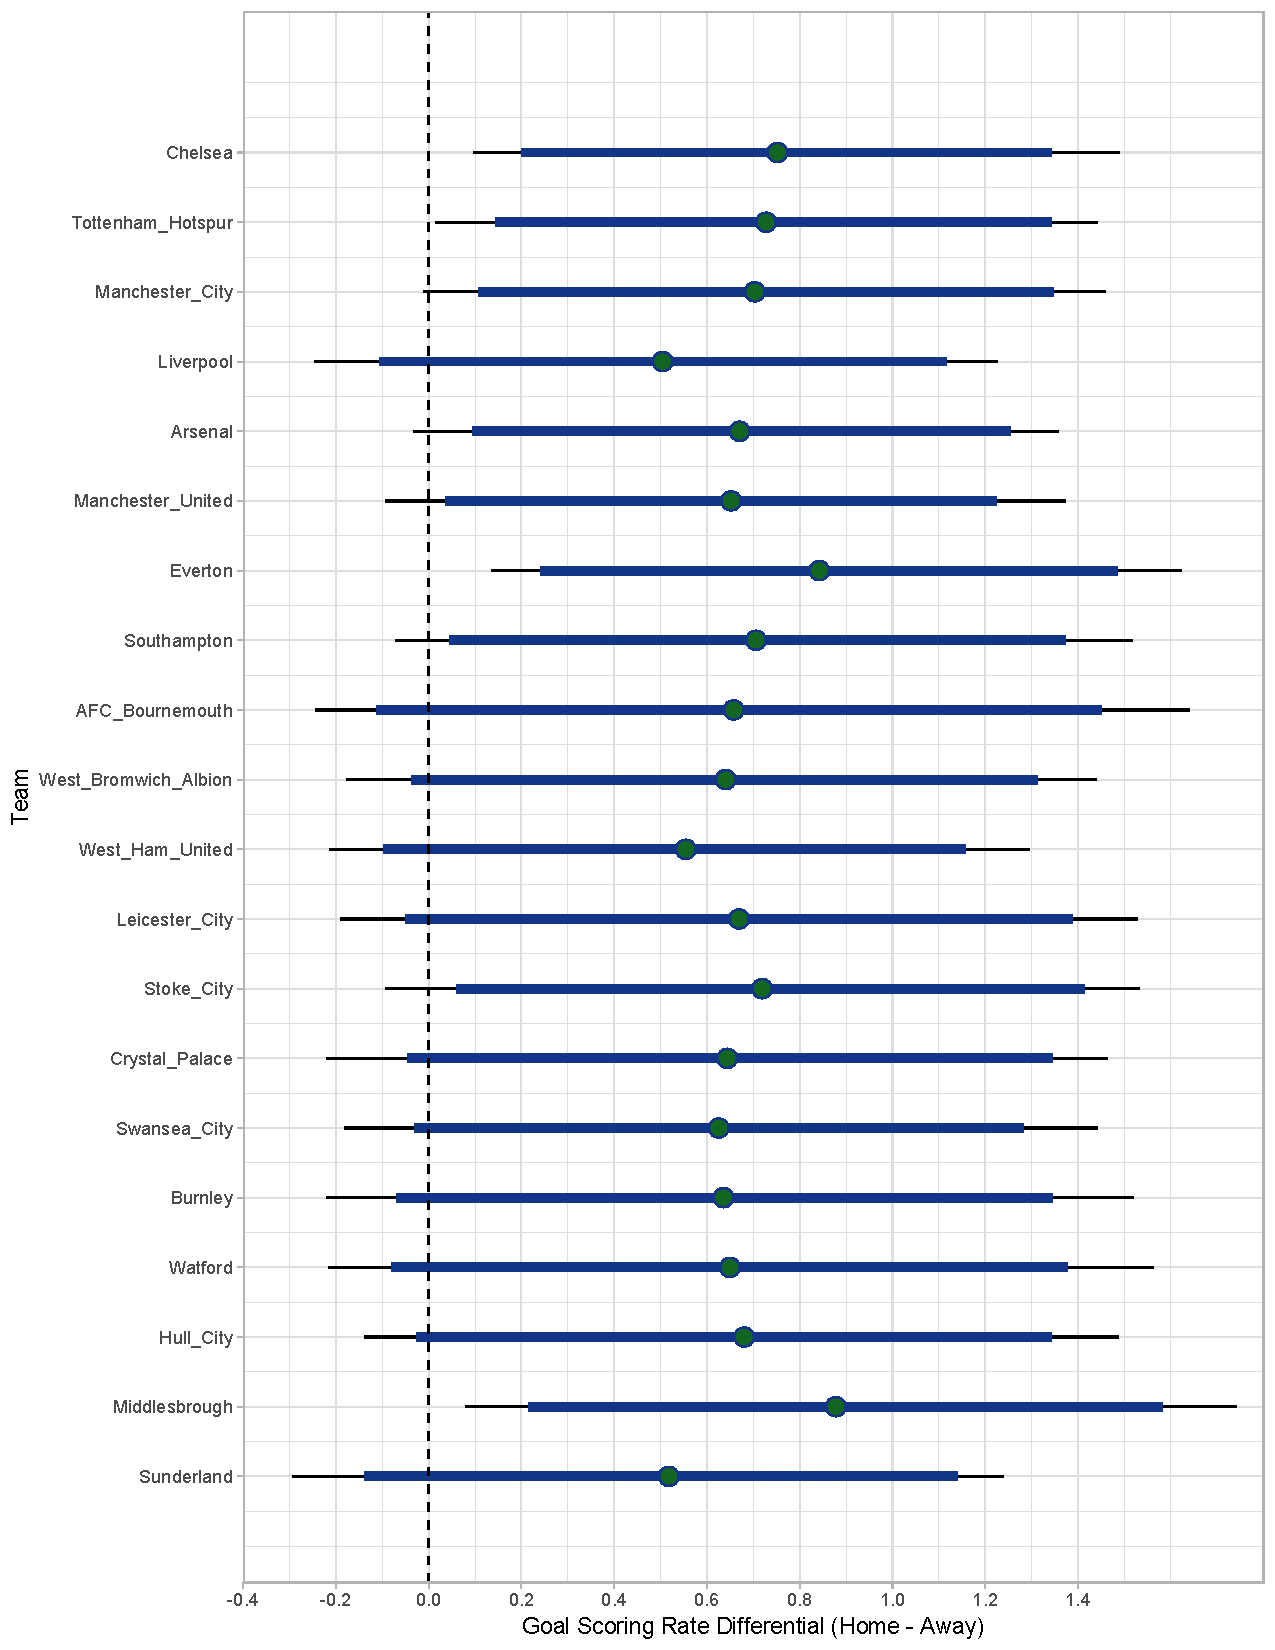
\includegraphics[width=0.90\linewidth]{HFA_EPL11.pdf}}
\label{fig7}
\end{figure}


\begin{acknowledgement}

We would like to thank ESPN FC for compiling the season-level club performance data and allow public access.

\end{acknowledgement}

\newpage

%\bibliographystyle{name}
\bibliography{Soccer}
\end{document}
